\documentclass[12pt,a4paper]{report}
\usepackage[utf8]{inputenc}
\usepackage{amsmath}
\usepackage{algorithm}
\usepackage{algpseudocode}
\usepackage{amssymb}
\usepackage{graphicx}
\usepackage{geometry}
\usepackage[hidelinks]{hyperref}  % For clickable references
\usepackage[capitalise]{cleveref}  % For intelligent cross-referencing
\usepackage[english]{babel}

\usepackage{makecell}
\usepackage{caption}
\usepackage{array}
\usepackage{listings}
\usepackage{titlesec}
\usepackage{hyperref}
\hypersetup{
	colorlinks=true,
	linkcolor=black,
	filecolor=black,      
	urlcolor=cyan,
	citecolor=black
}

\graphicspath{{C:/Users/frabb/OneDrive - Cal Poly/Documents (Cloud)/0 CALPOLY/000Thesis/Chapters/Images/}}

\geometry{
	top=1in,
	bottom=1in,
	left=1.5in,
	right=1in
}

% Remove space before equations only
\makeatletter
\g@addto@macro\normalsize{%
	\setlength\abovedisplayskip{-10pt}
	\setlength\abovedisplayshortskip{-10pt}
}
\makeatother

% Updated list settings
\usepackage{enumitem}
\setlist[itemize]{nosep, leftmargin=*}
\setlist[enumerate]{nosep, leftmargin=*}

% Remove space before lists
\usepackage{etoolbox}
\BeforeBeginEnvironment{itemize}{\vspace{-\baselineskip}}
\BeforeBeginEnvironment{enumerate}{\vspace{-\baselineskip}}

\setlength{\parskip}{\baselineskip}
\titlespacing*{\section}{0pt}{0pt}{0pt}
\titlespacing*{\section}{0pt}{0pt}{-10pt}
\titlespacing*{\subsection}{0pt}{0pt}{-10pt}

\captionsetup[table]{skip=0pt}

\usepackage{xcolor}

\definecolor{codegreen}{rgb}{0,0.6,0}
\definecolor{codegray}{rgb}{0.5,0.5,0.5}
\definecolor{codepurple}{rgb}{0.58,0,0.82}
\definecolor{backcolour}{rgb}{0.95,0.95,0.92}

\lstdefinestyle{mystyle}{
	backgroundcolor=\color{backcolour},   
	commentstyle=\color{codegreen},
	keywordstyle=\color{magenta},
	numberstyle=\tiny\color{codegray},
	stringstyle=\color{codepurple},
	basicstyle=\ttfamily\footnotesize,
	breakatwhitespace=false,         
	breaklines=true,                 
	captionpos=b,                    
	keepspaces=true,                 
	numbers=left,                    
	numbersep=5pt,                  
	showspaces=false,                
	showstringspaces=false,
	showtabs=false,                  
	tabsize=2
}

\lstset{style=mystyle}

\title{Tutorial}
\author{Jakob Frabosilio}
\date{\today}
\setcounter{chapter}{2}
\begin{document}
	
\chapter{Acoustic Positioning System} \label{chap:4c}
The acoustic positioning system is the core of the iSBL-SF algorithm. In this system, an acoustic pulse is sent by a transmitter and recorded by receivers on the iSBL array. The time shift between the signals from each receiver is calculated, and these shifts are used to estimate the transmitter’s position relative to the iSBL array using an acoustic propagation model. Chapter \ref{chap:4c} describes how the orientation estimate of the platform is determined (and how dead-reckoning is introduced), and Chapter \ref{chap:5c} details how Kalman filters are used to get the best position estimate by combining multiple data sources. This chapter describes only the acoustic positioning system, the central component of this thesis.

The first section in this chapter is dedicated to previous implementations of acoustic positioning systems, and how the iSBL approach differs from them. Next, the mechanical design of the receiver array is discussed. The electrical design of the acoustic positioning system, including the wiring diagram of the full iSBL array, is then detailed. The ultrasonic receivers receive their own section, where the design and manufacturing of the active band-pass filter PCB is explained. Then, the assembly of the full iSBL array is described, followed by the hardware and software design of the transmitter system. The final three sections are devoted to the software of the acoustic positioning system: how an acoustic pulse is detected and recorded, how the time shift between signals is calculated, and finally, how a position estimate is formed.

\section{Previous Works} \label{sec:3s1}
Acoustic positioning systems are not a new invention, and many different designs have been tested and implemented over the years. The rise of autonomous underwater vehicles has accelerated research into this field. In this section, the history of acoustic positioning systems is recounted, and the primary difference among these systems (the baseline length) is described. Lastly, similar implementations to this thesis are detailed.

\subsection{History of Acoustic Positioning Systems} \label{ssec:3s1s1}
The first known underwater acoustic positioning system was deployed in 1963, when a short baseline acoustic positioning system was used to guide the bathyscape \emph{Trieste 1} to the wreck of the US nuclear submarine USS \emph{Thresher}. The system barely worked, only guiding the \textit{Trieste} to the wreck once after ten unsuccessful attempts. The technology advanced as commercial applications became evident; oil and gas exploration in the 1970s was a primary driver for advancement. In 1998, a long baseline acoustic positioning system was used by a salvage company to navigate a debris field of a sunken WW2 Japanese submarine at 5240m deep. Current advancements in the field are primarily driven by the oil and gas industry, academic research, and defense industry applications \cite{apomab}.

\begin{figure}[htbp]
	\centering
	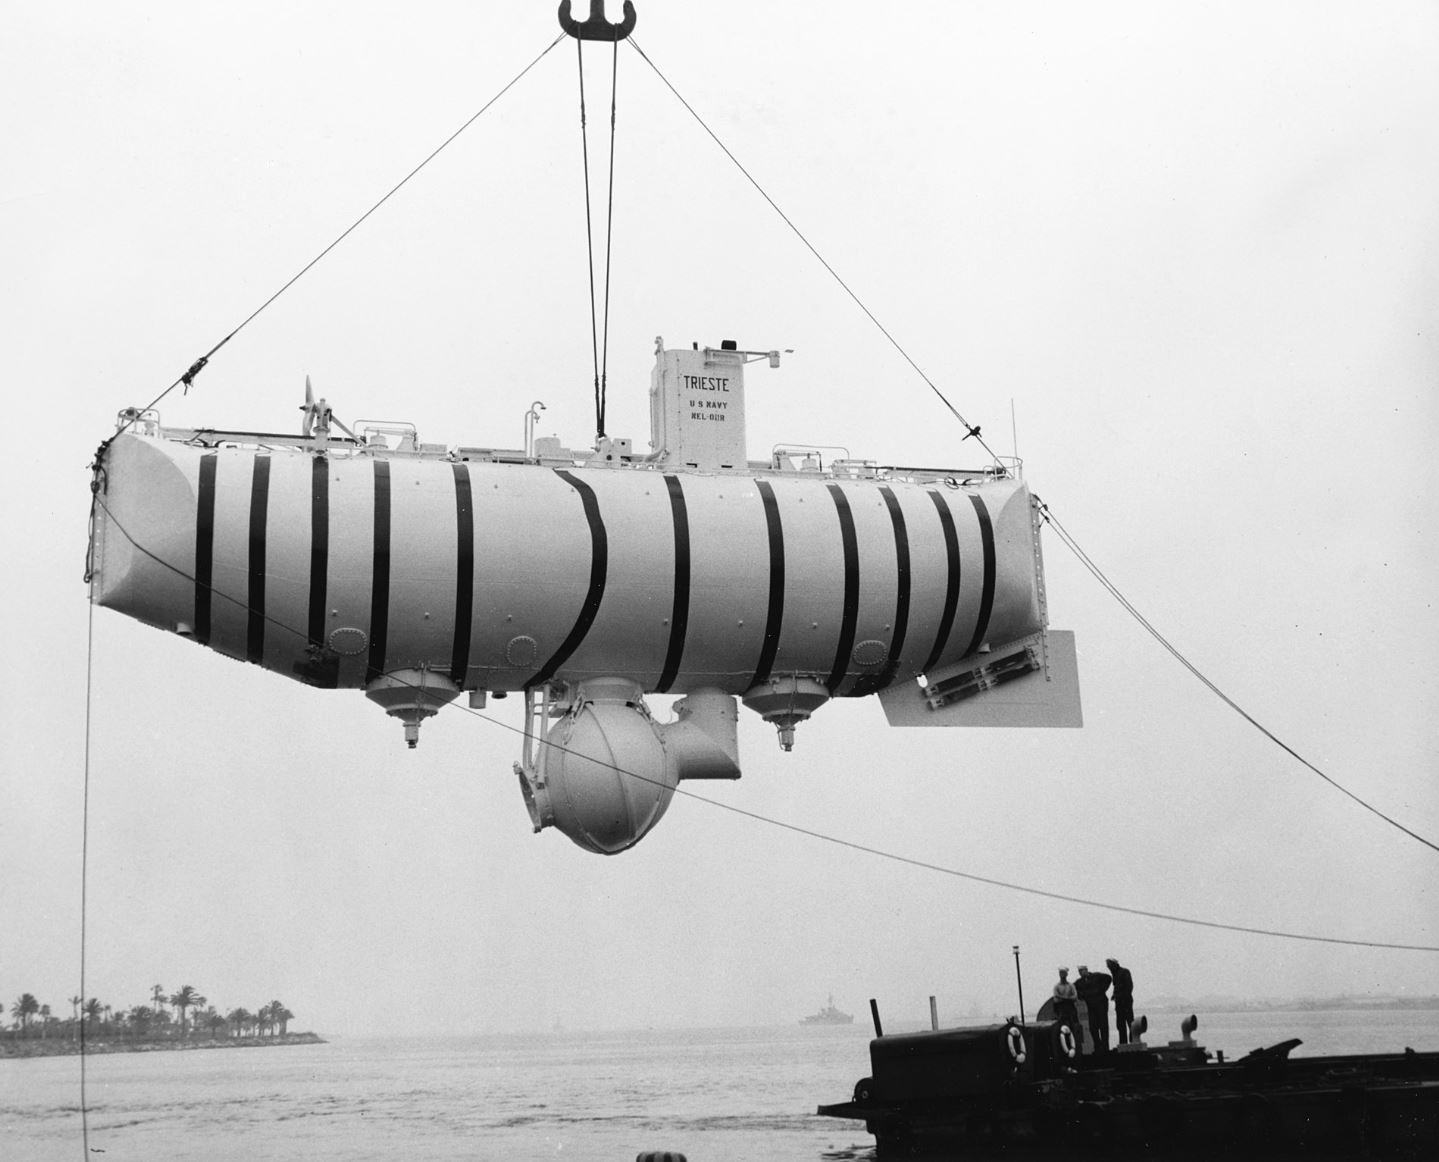
\includegraphics[width=0.5\textwidth]{trieste}
	\caption{Bathyscape \textit{Trieste 1}, which used the first short baseline acoustic positioning system to locate a nuclear submarine wreck \cite{apomab}}
	\label{fig:trieste}
\end{figure}

\section{Active Band-Pass Filter Design} \label{sec:3s4}
This implementation is designed to work with 40kHz audio signals. This frequency was chosen for a few reasons:
\begin{itemize}[noitemsep,topsep=0pt,]
	\item The above-water frequency should be similar to the planned underwater system’s frequency to allow for simple future implementation
	\item The audible range should be avoided to minimize disturbance to marine animals (see Section \ref{sec:6s4} for more details on the underwater system extrapolation)
	\item Lower frequencies require lower ADC sampling rates to record a single wave
	\item Lower audio frequencies attentuate much less rapidly in seawater compared to higher frequencies (see Figure \ref{fig:attenuation})
	\item 40kHz is a very common frequency for air-based ultrasonic transducers, and fairly common in water-based ultrasonic transducers
\end{itemize}

\begin{lstlisting}[language=C++]
	message_int ++;			// pick the next number
	message_int %= 256;		// between 0 and 255 (8-bit length),
	message_char = (char)message_int;		// and save it as a char
	
	// save in the last 8 bits of message_string
	for(int i = 8; i > 0; i--){				
		message_string[14-i] = (message_int >> (i-1)) & 1;
	}
	
	message_string[0] = 1; 	// initialize the message with a header
	message_string[1] = 1;
	message_string[2] = 1;
	message_string[3] = 1;
	message_string[4] = 0;
	message_string[5] = 0;
\end{lstlisting}

\begin{table}[htbp]
	\centering
	\caption{Truth table for motor driver}
	\label{tab:truth}
	\begin{tabular}{|c|c|c|c|}
		\hline
		Logic level, InA & Logic level, InB & Voltage, Out1 & Voltage, Out2 \\
		\hline
		0 & 0 & 0V & 0V \\
		\hline
		0 & 1 & +12V & 0V \\
		\hline
		1 & 0 & 0V & +12V \\
		\hline
		1 & 1 & +12V & +12V \\
		\hline
	\end{tabular}
\end{table}

\begin{equation} \label{eq:3eq4}
	\mathbf{q} = q_0 + iq_1 + jq_2 + kq_3
\end{equation}

\begin{equation} \label{eq:3e4q4}
	\mathbf{q}_n = (1 - \gamma) \mathbf{q}_{acc/mag} + \gamma (\mathbf{q}_{n-1} + \delta t \times \mathbf{q}_{gyro})
\end{equation}


\begin{algorithm}
	\caption{Hooke-Jeeves Search Algorithm in \textbf{n} Dimensions} \label{alg:hooke-jeeves-3d}
	\begin{algorithmic}[1]
		\Require InitialPosition, MaxIterations, MinResidual, MinSpacing, ScaleFactor, InitialSpacing
		\Ensure OptimizedPosition
		
		\State $position \gets InitialPosition_{\mathbf{n} \times 1}$
		\State $newPosition \gets InitialPosition_{\mathbf{n} \times 1}$
		\State $residual \gets \infty$
		\State $spacing \gets InitialSpacing \times ScaleFactor$
		\State $iteration \gets 0$
		\State $newDirectionNeeded \gets false$
		\State $direction \gets \mathbf{0}_{\mathbf{n} \times 1}$
		
		\While{$iteration < MaxIterations$ \textbf{and} $residual > MinResidual$ \textbf{and} $spacing > MinSpacing$}
		\If{$newDirectionNeeded$}
		\State $spacing \gets spacing / ScaleFactor$
		\For{each dimension $\mathbf{d}$ in $\mathbf{n}$}
		\State $direction \gets \mathbf{0}_{\mathbf{n} \times 1}$
		\State $direction(\mathbf{d}) \gets 1$
		\State $testPosition \gets position + direction \times spacing$
		\State $residualList(2\mathbf{d}) \gets$ CalculateResidual($testPosition$)
		\State $testPosition \gets position - direction \times spacing$
		\State $residualList(2\mathbf{d}+1) \gets$ CalculateResidual($testPosition$)
		\EndFor
		\If{min$(residualList) < residual$}
		\State $direction \gets \arg\!\min_{direction}(residualList)$
		\State $residual \gets$ min$(residualList)$
		\State $position \gets position + direction \times spacing$
		\State $newDirectionNeeded \gets false$
		\Else
		\State $newDirectionNeeded \gets true$
		\EndIf
		\Else
		\State $prevResidual \gets residual$
		\State $newPosition \gets position + direction \times spacing$
		\State $residual \gets$ CalculateResidual($newPosition$)
		\If{$residual < prevResidual$}
		\State $position \gets newPosition$
		\Else
		\State $residual \gets prevResidual$
		\State $newDirectionNeeded \gets true$
		\EndIf
		\EndIf
		\State $iteration \gets iteration + 1$
		\EndWhile
		
		\Return $position$
	\end{algorithmic}
\end{algorithm}

\bibliographystyle{IEEEtran}
\bibliography{../thesis}
	
\end{document}